\section*{Method}
\label{Method}
%
In order to know whether or not the BTL model and the Preference Tree-model can be applied to the data shown in \autoref{tab:data}, it is first necessary to check for transitivity in the data. In other words how reliable and consistent the data is. The cumulative preference matrix is a pooled data matrix meaning it contains data from all the participants deemed sufficiently consistent. This is typically done using a Chi-square-test. Now a problem could arise because it is unknown whether the pooled subjects have shown an opposite decision behaviour or not eg. chosen high risk where others low risk. If that is the case, then the preference matrix becomes inconsistent. Before it is possible to do the transitivity check, it is necessary to calculate the probability of a stimulus being rated as high risk. See \autoref{eq:probability}.
%
\begin{equation}
p = \frac{freq}{n}
\label{eq:probability}
\end{equation}
\noindent
%
Here \textit{freq} is the frequency that a drug has been rated as having the highest health risk (the pooled preference matrix, \autoref{tab:data}) and \textit{n} is the number of test subjects. Thereafter it is needed to check every combination of the stimuli for transitivity violations. There are no set rules but a rough estimate of when the probabilistic choice models holds is shown in \autoref{tab:trans_violations}:
%
\begin{table}[H]
\centering
\begin{tabular}{@{}ll@{}}
\toprule
Transitivity violations                                    & Expected                                      \\ \midrule
None or few SST violations                                 & BTL may fit                                   \\
Some SST violations and few MST violations                 & Preference Tree might fit (Not BTL)            \\
Considerable SST and MST but few WST violations & Possible to rank order (no model will fit) \\ \bottomrule
\end{tabular}
\caption{General estimates of the outcome of probabilistic choice models considering the amount of weak (WST), moderate (MST) and strong (SST) transitivity violations.}
\label{tab:trans_violations}
\end{table}
\noindent
%
Consider three stimuli: \textit{a}, \textit{b}, and \textit{c}. If it is observed that $p_{ab} \geq 0.05$ and $p_{bc} \geq 0.05$, in other words if the probability of \textit{a} being rated as more unpleasant compared to \textit{b} and \textit{b} more unpleasant compared to \textit{c}. Then Weak Stochastic Transitivity (WST) holds when $p_{ac} \geq 0.05$. It is considered a WST violation if $p_{ac} < 0.05$. The same logic applies to MST and SST. If $p_{ac}$ is bigger than or equal to the minimum value in $p_{ab}$ and $p_{bc}$, MST holds ($p_{ac}\geq min(p_{ab};p_{bc}$). It is a violation if not. For SST, $p_{ac}$ is compared to the maximum value of both $p_{ab}$ and $p_{bc}$. If $p_{ac}$ is not bigger or equal to these values, it counts as an SST violation ($p_{ac}< max(p_{ab};p_{bc}$.)

Luckily, with the help of Matlab it is not needed to perform every single comparison by hand. A loop was written which identified the number of WST, MST and SST violations respectively:\\
\pagebreak
%butt-rape in 3... 2... 1... 
\texttt{
\hspace{1mm}WST = 0; \\ 
\hspace{1mm}MST = 0; \\ 
\hspace{1mm}SST = 0; \\ 
\hspace{1mm}Count = 0; \\ 
\noindent
\hspace{1mm} \\ 
\hspace{1mm}\textcolor{blue}{for} a = 1:6; \\ 
\hspace{1mm}\indent \textcolor{blue}{for} b = 1:6; \\ 
\hspace{1mm}\indent \indent \textcolor{blue}{for} c = 1:6; \\ 
\hspace{1mm}\indent \indent \indent \textcolor{blue}{if} (a~=b)\&\&(b~=c)\&\&(a~=c); \textcolor{green}{\%avoids comparing diagonal (0) }\\ 
\hspace{1mm}\indent \indent \indent \indent \textcolor{blue}{if} p\_model(a,b)$>$=0.5 \&\& p\_model(b,c) $>$=0.5; \\ 
\hspace{1mm}\indent \indent \indent \indent \indent Count = Count+1; \\ 
\hspace{1mm}\indent \indent \indent \indent \indent \textcolor{blue}{if} p\_model(a,c)$<$0.5; \textcolor{green}{\%checks for WST violations }\\ 
\hspace{1mm}\indent \indent \indent \indent \indent \indent \indent WST = WST+1; \textcolor{green}{\%counts number of violations }\\ 
\hspace{1mm}\indent \indent \indent \indent \indent \indent \textcolor{blue}{end} \\ 
\hspace{1mm}\indent \indent \indent\indent \indent \indent \indent\indent \textcolor{green}{\%checks for MST violations }\\ 
\hspace{1mm}\indent \indent \indent \indent \indent \indent \indent \textcolor{blue}{if} p\_model(a,c) $<$ min(p\_model(a,b),p\_model(b,c)); \\ 
\hspace{1mm}\indent \indent \indent \indent \indent \indent \indent \indent MST = MST+1; \textcolor{green}{\%counts number of violations }\\ 
\hspace{1mm}\indent \indent \indent \indent \indent \indent \indent \textcolor{blue}{end} \\ 
\hspace{1mm}\indent \indent \indent \indent \indent\indent \indent \indent \textcolor{green}{\%checks for SST violations }\\ 
\hspace{1mm}\indent \indent \indent \indent \indent \indent \indent \indent \textcolor{blue}{if} p\_model(a,c) $<$ max(p\_model(a,b),p\_model(b,c)); \\ 
\hspace{1mm}\indent \indent \indent \indent \indent \indent \indent \indent \indent SST = SST+1;\textcolor{green}{\%counts number of violations }\\ 
\hspace{1mm}\indent \indent \indent \indent \indent \indent \indent \indent \textcolor{blue}{end} \\ 
\hspace{1mm}\indent \indent \indent \indent \indent \indent \indent \textcolor{blue}{end} \\ 
\hspace{1mm}\indent \indent \indent \indent \indent \indent \textcolor{blue}{end} \\ 
\hspace{1mm}\indent \indent \indent \indent \indent \textcolor{blue}{end} \\ 
\hspace{1mm}\indent \indent \indent \indent \textcolor{blue}{end} \\ 
\hspace{1mm}\indent \indent \indent \textcolor{blue}{end} \\ 
}

%
%\begin{figure}[H]
%\centering
%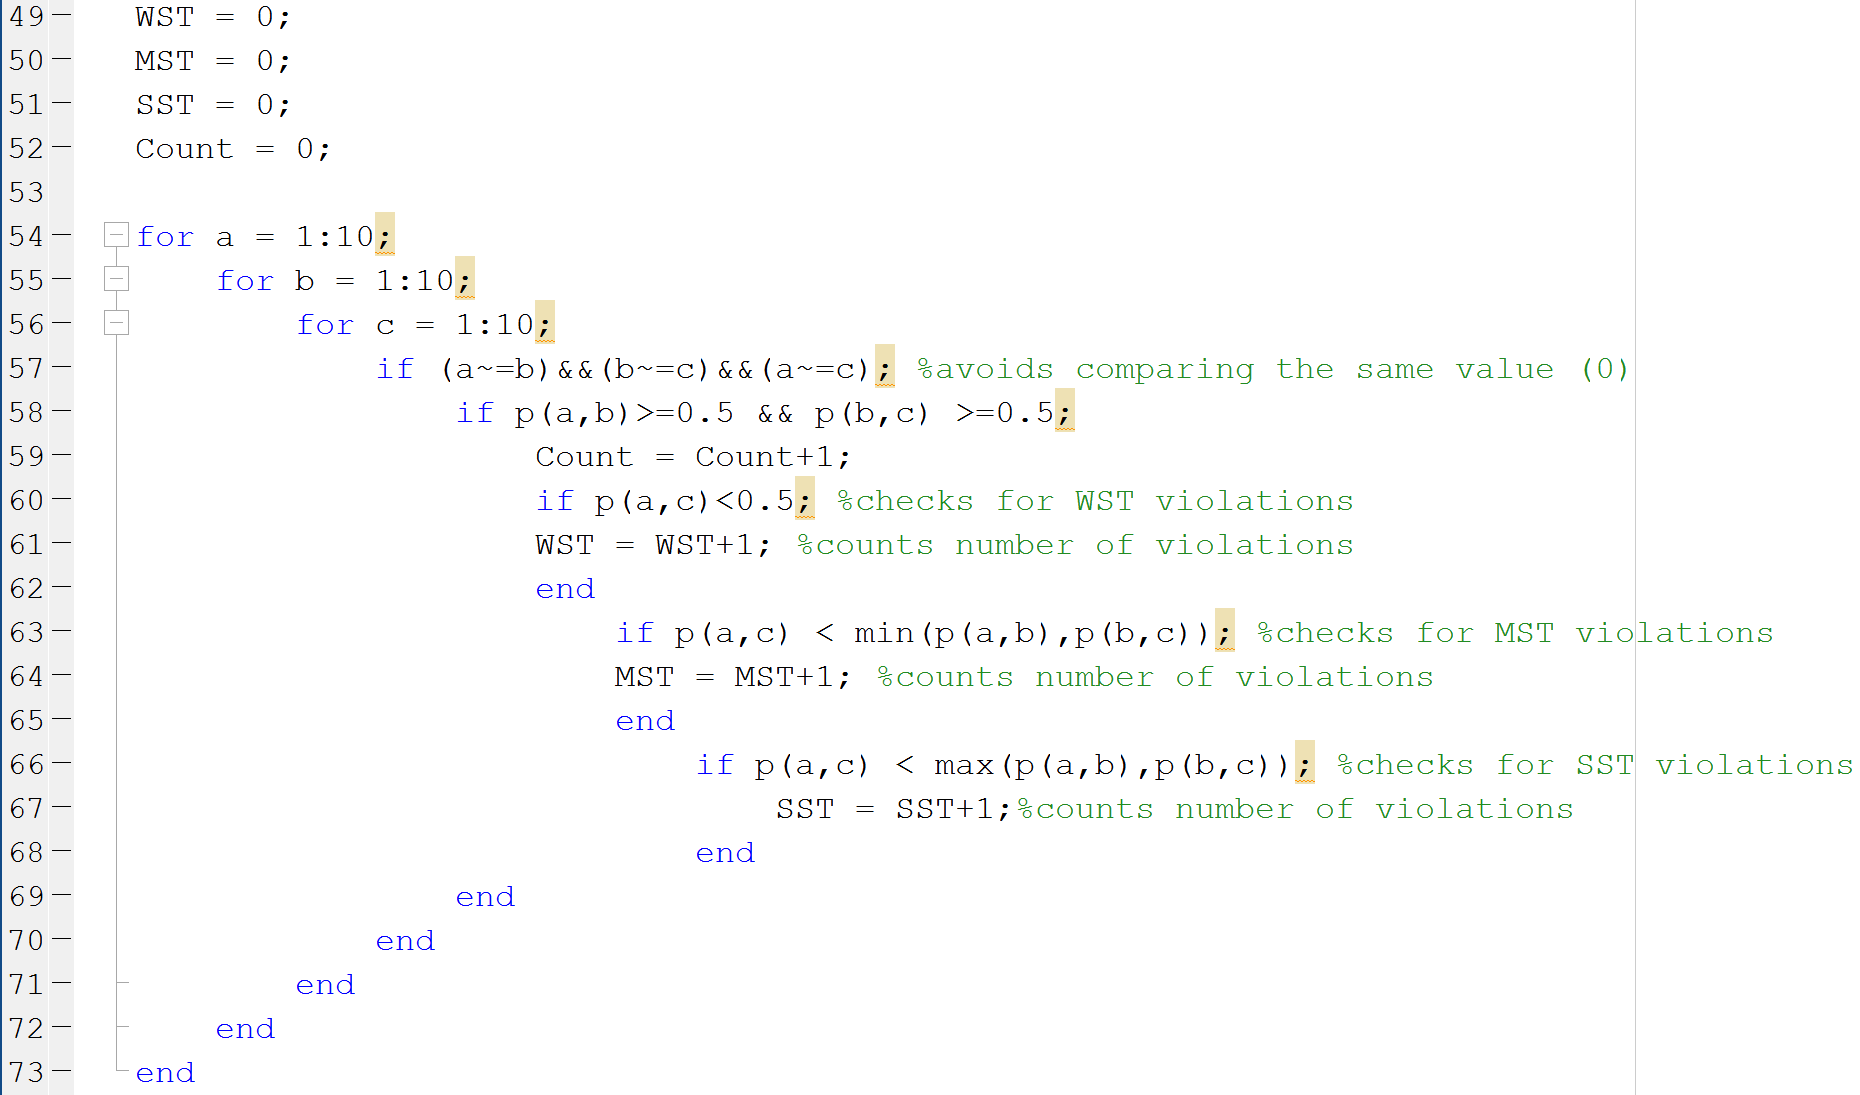
\includegraphics[width = \textwidth]{Figure/loop} 
%\caption{Loop used to calculate WST, MST and SST violations.}
%\label{fig:loop}
%\end{figure}
%\noindent
%
\subsection*{Bradley-Terry-Luce (BTL)}
The probabilistic method used called the BTL-model has a simple model structure, where only one attribute distinguish the stimuli. The model checks for transitivity in data containing pairwise comparisons and is able to predict the outcome of the comparison. See \autoref{eq:BTL}.
%
\begin{equation}
P_{ab} =\frac{v(a)}{v(a)+v(b)} 
\label{eq:BTL}
\end{equation}
%
$P_{ab}$ is the probability of drug \textit{a} being rated to be of higher health risk than drug \textit{b}. \textit{v(a)} and \textit{v(b)} denotes the scale values of drug \textit{a} and \textit{b}.

In order to get estimates of the scale values, one has to maximise the likelihood of the data seen in \autoref{tab:data}. This is done given the model in \autoref{eq:max_likelyhood}: 
%
\begin{equation}
L(D|\Theta_{model}) = \prod_{i<j} p_{ij} ^{n_{ij}}\cdot(1- p_{ij})^{n-n_{ij}}
\label{eq:max_likelyhood}
\end{equation}
\noindent 
%
Where \textit{n} is the number of comparisons, which is equal to the amount of test subjects in this case (\textit{n=48}) and $n_{ij}$ is the frequency of how many times the drug in row \textit{i} was rated as being of higher health risk than the drug in column \textit{j}. $P_{ij}$ is the preference probability and is estimated using \autoref{eq:BTL}. 

\subsection*{Preference Tree}
%
The Preference Tree has a more complex structure than the BTL-model, where it has subgroups of attributes. The model assumes the relationship shown in \autoref{eq:PT} between scale values and the probability the stimuli \textit{v(a)} is chosen over \textit{v(b)}.
%
\begin{equation}
P_{ab} =\frac{v(a'-b')}{v(a'-b')+v(b'-a')} 
\label{eq:PT}
\end{equation}
\noindent
%
$P_{ab}$ is the probability of drug \textit{a} being rated to be of higher health risk than drug \textit{b}. \textit{v(a'-b')} is the scale value for the attribute(s) that \textit{a} does not share with \textit{b} and last is \textit{v(b'-a')} which is the scale value for the attribute(s) that \textit{b} does not share with \textit{a}.

In order to get estimates of the scale values, one has to maximise the likelihood (\textit{L}) of the data seen in \autoref{tab:data}. This is done given the model in \autoref{eq:max_likelyhood} and this is exactly like it was done for for the BTL-model. 
\\\\
For estimation the likelihood the \textit{fOptiPt.m} Matlab function has been developed by Florian Wickelmaier and Christian Schmid \parencite{Wickelmaier2004}. The function requires two mandatory input, \textit{M} and \textit{A}, where \textit{M} is the paired comparison matrix shown in \autoref{tab:data}, and \textit{A} is a cell array with length corresponding to the number of stimuli, which is 10. Further there is an optional input, \textit{s}, which denotes the starting values for the estimation routine. The search algorithm starts at $\frac{1}{k}$ for each parameter value, where \textit{k} is the number of parameters, if \textit{s} is not specified. In the case with both the BTL-model and Preference Tree, \textit{s} is not specified nor is it used.
\vfill